
\section{Appendix: Provably Secure Append-only Accumulator}

This section describes the core data structure for implementing the Unicity's Aggregation Layer in trustless way.

Trustless append only accumulator is consistent, if during insertion of a batch of updates there were no changes or deletions of existing leaves. The data structure implements other usual functions like inclusion proofs and non-inclusion proofs.

The size of consistency proof depends on the size of addition batch and logarithm of capacity. If we denote batch size as $k$ and depth $d$, then size of consistency proof is $O(k \cdot d)$, where $d \approx \log(capacity)$.

By using a cryptographic SNARK (a zero knowledge proof with certain properties), the size of consistency proof can be further reduced to constant size.

After every addition batch, the root of aggregation layer is certified by the BFT Finality Gadget, ensuring its uniqueness and immutability. This provides a useful trust anchor for consistency proofs, inclusion proofs, and non-inclusion proofs.

\subsection{Proof of Consistency}

We have $i$th batch of insertions $B = (k_1, k_2, \dots, k_j)$, where $k$ is an inserted item; all executed during a round of operation. Root hash before the round is $r_{i-1}$, and after the round is $r_i$. The accumulator is implemented as a Sparse Merkle Tree (SMT).

The consistency proof generation for batch $B_i$ works as follows:

\begin{itemize}
    \item Insert the new SMT leaves in $B_i$,
    \item Starting from the newly inserted leaves, for each sibling hash necessary to compute the root of the tree, we record sibling's path and sibling's value as the proof. Let's denote the set as $s_i$.
    \item Record $(B_i, r_{i-1}, r_i, s_i)$.
\end{itemize}

Proof verification works as follows:
\begin{itemize}
    \item authenticate $r_{i-1}, r_i$
    \item Build an incomplete SMT tree: for each item in $B_i$, we insert the value of empty leaf at appropriate position,
    \item All necessary siblings necessary to compute the root are available in $s_i$. Compute the root, compare with $r_{i-1}$, if not equal then proof is not valid.
    \item Build again an incomplete SMT tree, for each item in $B_i$, we insert the value of each key into appropriate position.
    \item Compute the root based on siblings in $s_i$. If root is not equal to $r_i$ then proof is not valid.
    \item Proof is valid if the checks above passed.
\end{itemize}

This shows that given authentic $s_{i-1}, s_i$, the keys in $B_i$ were empty before the insertion batch, and after execution of insertion batch the values in $B_i$ were recorded at the positions defined by respective keys, and there were no other changes.


\subsection{SNARK based Proof of Consistency}

Statement to be proved is the verification algorithm sketched above. Instance is defined by the root of trust and insertions, $I = ((r_i, r_{i-1}),B_i)$. Witness $\omega = (s_i, s'_i)$ is the secret in zero knowledge, but for our use-case, it is not necessary to keep the witness secret.

The statement is implemented as a constraint system $R$ using the CIRCOM domain specific language. The witness is generated based on $s_i, B_i$, and supplemented by control wires defining how individual hashing blocks in the circuit are connected together and to the inputs. If all constraints are satisfied, then the proof is valid.

\begin{figure}[htb]
    \centering
    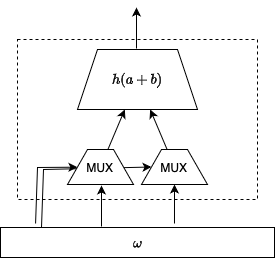
\includegraphics[width=0.33\textwidth]{smt-circuit-cell.drawio}
    \caption{A cell of the ZK circuit}
    \label{fig:zk-circuit-cell}
\end{figure}

\begin{figure}[htb]
    \centering
    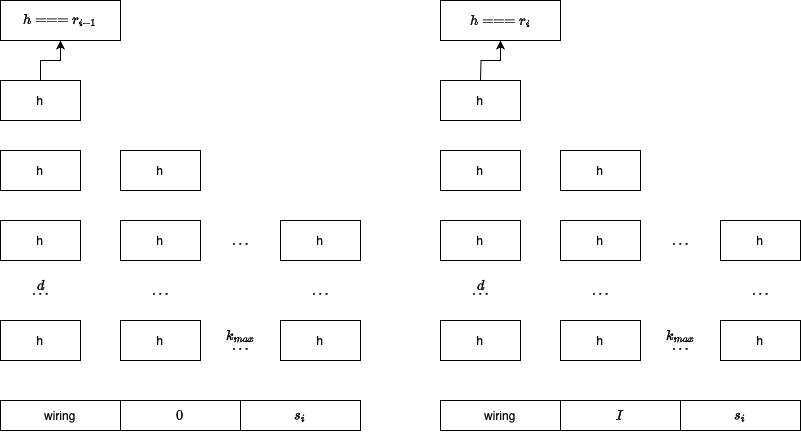
\includegraphics[width=\textwidth]{smt-circuit.drawio}
    \caption{The ZK circuit for SMT consistency verification; cells are connected together and to the input vector based on pre-generated wiring signals}
    \label{fig:zk-circuit}
\end{figure}

The proving backend is Groth 2016\footnote{\url{https://eprint.iacr.org/2016/260}} with conveniently small proof size. The proving time depends on the depth of SMT and the maximum size of the insertion batch. Importantly, the proving effort does not depend on the total size/capacity of SMT, enabling fairly large instantiations.

If the layer above verifies proofs of consistency, then Unicity aggregation layer is trustless. Still, some redundancy (at least one node able to persist the data structure) is required for data availability.
